\newpage
\section{GIẢI BẤT PHƯƠNG TRÌNH BẬC HAI MỘT ẨN}
\subsection{LÝ THUYẾT CẦN NHỚ}
\subsubsection{Bất phương trình bậc hai một ẩn}
\begin{boxdn}
\begin{itemize}
	\item \textit{Bất phương trình bậc hai một ẩn } $x$ là bất phương trình có một trong các dạng $ax^2+bx+c\le 0$, $ax^2+bx+c<0$, $ax^2+bx+c\ge 0$, $ax^2+bx+c> 0$, với $a \ne 0$.
	\item \textit{Nghiệm } của bất phương trình bậc hai là các giá trị của biến $x$ mà khi thay vào bất phương trình ta được bất đẳng thức đúng. 
	\item \textit{Giải bất phương trình bậc hai } là tìm tập hợp các nghiệm của bất phương trình đó.
\end{itemize}
\end{boxdn}

\subsubsection{Giải bất phương trình bậc hai một ẩn}
\begin{boxdn}
Giải bất phương trình bậc hai một ẩn có dạng $f(x)=ax^2+bx+c>0$.\\
\textbf{Cách 1.} Sử dụng định lý về dấu của tam thức bậc hai.
\begin{itemize}
	\item \textit{Bước 1:} Xác định dấu của hệ số $a$ và tìm nghiệm của $f(x)$ (nếu có).
	\item \textit{Bước 2:} Sử dụng định lý về dấu của tam thức bậc hai để tìm tập hợp những giá trị của $x$ sao cho $f(x)$ mang dấu \lq\lq$+$\rq\rq.
\end{itemize}
\textbf{Cách 2.} Sử dụng đồ thị.\\
Dựa vào parabol $y=ax^2+bx+c$ tìm tập hợp những giá trị của $x$ ứng với phần parabol đó nằm phí trên trục hoành.
\box{dn}
\begin{luuy}
	Các bất phương trình bậc hai có dạng $f(x)<0$, $f(x)\le 0$, $f(x)\ge 0$ được giải bằng cách tương tự.
\end{luuy}
\subsection{PHÂN LOẠI VÀ PHƯƠNG PHÁP GIẢI TOÁN}
\begin{dang}{Giải bất phương trình bậc hai một ẩn}
Phương pháp: sử dụng định lý về dấu của tam thức bậc hai hoặc đồ thị
\end{dang}
\begin{vd}%[0D4Y5-2]%[Dự án đề cương 3 Khối NH25-26- Đợt 1- Nguyễn Cường]
	Giải các bất phương trình sau	
	\begin{multicols}{3}
		\begin{enumerate}
			\item $-3x^2+2x+1<0$.
			\item $x^2+x-12\ge 0$.
			\item $-x^2+x+6 \le 0$.
			\item $-x^2+x-5<0$.
			\item $x^2-2x-4>0$.
			\item $4x^2+4x+1>0$.
		\end{enumerate}
	\end{multicols}
	\loigiai{
		\begin{enumerate}
			\item Ta có $-3x^2+2x+1=0 \Leftrightarrow x=-\dfrac{1}{3}$ hoặc $x=1$.\\
			Bảng xét dấu
			\begin{center}
				
\begin{tikzpicture}
					\tkzTabInit[lgt=3,espcl=2]
					{$x$ /1.2, $-x^2+4x+5$ /0.8}
					{$-\infty$,$-\dfrac{1}{3}$,$1$,$+\infty$}
					\tkzTabLine{ ,-,$0$,+,$0$,-,}
				\end{tikzpicture}
			\end{center}
			Dựa vào bảng xét dấu, ta có tập nghiệm của bất phương trình là $S=\left(-\infty;-\dfrac{1}{3}\right)\cup (1;+\infty)$.
			\item Ta có $x^2+x-12=0 \Leftrightarrow x=3$ hoặc $x=-4$.\\
			Bảng xét dấu
			\begin{center}
				
\begin{tikzpicture}
					\tkzTabInit[lgt=3,espcl=2]
					{$x$ /0.8, $x^2+x-12$/0.8}
					{$-\infty$,$-4$,$3$,$+\infty$}
					\tkzTabLine{ ,+,$0$,-,$0$,+,}
				\end{tikzpicture}
			\end{center}
			Dựa vào bảng xét dấu, ta có tập nghiệm của bất phương trình là $S=(-\infty;-4] \cup [3;+\infty)$.	
			\item Ta có $-x^2+x+6=0 \Leftrightarrow x=-2$ hoặc $x=3$.
			Bảng xét dấu
			\begin{center}
				
\begin{tikzpicture}
					\tkzTabInit[lgt=3,espcl=2]
					{$x$ /0.8, $-x^2+x+6$ /0.8}
					{$-\infty$,$-2$,$3$,$+\infty$}
					\tkzTabLine{ ,-,$0$,+,$0$,-,}
				\end{tikzpicture}
			\end{center}
			Dựa vào bảng xét dấu, ta có tập nghiệm của bất phương trình là $S=\left(-\infty;-2\right]\cup [3;+\infty)$.
			\item $-x^2+x-5=0$ vô nghiệm nên ta có bảng xét dấu
			\begin{center}
				
\begin{tikzpicture}
					\tkzTabInit[lgt=3,espcl=5]
					{$x$ /0.8, $-x^2+x-5$ /0.8}
					{$-\infty$,$+\infty$}
					\tkzTabLine{ ,-,}
				\end{tikzpicture}
			\end{center}
			Dựa vào bảng xét dấu, ta có tập nghiệm của bất phương trình là $\mathbb{R}$.
			\item Ta có $x^2-2x-4=0\Leftrightarrow x=1-\sqrt{5}$ hoặc $x=1+\sqrt{5}$.\\
			Bảng xét dấu
			\begin{center}
								
\begin{tikzpicture}
					\tkzTabInit[lgt=3,espcl=2]
					{$x$ /0.8, $x^2-2x-4$ /0.8}
					{$-\infty$,$1-\sqrt{5}$,$1+\sqrt{5}$,$+\infty$}
					\tkzTabLine{ ,+,$0$,-,$0$,+,}
				\end{tikzpicture}
			\end{center}
			Dựa vào bảng xét dấu, ta có tập nghiệm của bất phương trình là $\left(-\infty;1-\sqrt{5}\right)\cup \left(1+\sqrt{5};+\infty\right)$.
			\item Ta có $4x^2+4x+1=0\Leftrightarrow x=-\dfrac{1}{2} $.\\
			Bảng xét dấu
			\begin{center}
				
\begin{tikzpicture}
					\tkzTabInit[lgt=3,espcl=2]
					{$x$ /1.2, $4x^2+4x+1$ /0.8}
					{$-\infty$,$-\dfrac{1}{2}$,$+\infty$}
					\tkzTabLine{ ,+,$0$,+,}
				\end{tikzpicture}
			\end{center}
			Tập nghiệm của bất phương trình là $\mathbb{R}\setminus\left\{-\dfrac{1}{2}\right\}$.
			
		\end{enumerate}
	}
\end{vd}
\begin{vd}%[Dự án đề cương 3 Khối NH25-26- Đợt 1- Nguyễn Cường]
	Tìm nghiệm của bất phương trình $ax^2+bx+c>0$, với đồ thị $f(x)=ax^2+bx+c$ được cho ở mỗi hình bên:\\
	\begin{enumerate}
		\item 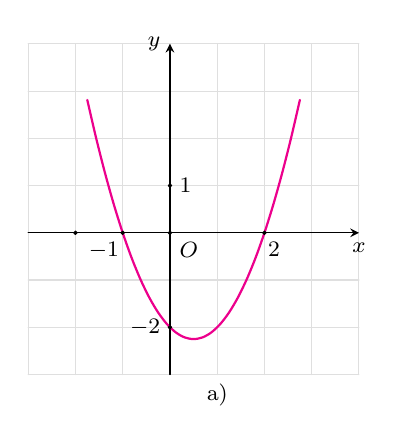
\begin{tikzpicture}[scale=.6, font=\footnotesize, line join=round, line cap=round,>=stealth]
		\draw[gray!50,opacity=.5](-3,-3)grid(4,4);
		\draw[->](-3,0)--(0,0)node[below right]{$O$}--(4,0)node[below]{$x$};
		\draw[->](0,-3)--(0,4)node[left]{$y$};
		\draw[smooth,domain=-1.75:2.75,thick, magenta]plot(\x,{(\x)^2-(\x)-2});
		\draw (1,-3)node[below]{a)};
		\draw(0,1)node[right]{$1$};
		\draw(0,-2)node[left]{$-2$};
		\draw(-1.4,0)node[below]{$-1$};
		\draw(2.2,0)node[below]{$2$};
		\foreach \x in {-2,-1,0,2}\draw[fill](\x,0)circle(1pt);
		\foreach \x in {-2,1}\draw[fill](0,\x)circle(1pt);
	\end{tikzpicture}
	\item 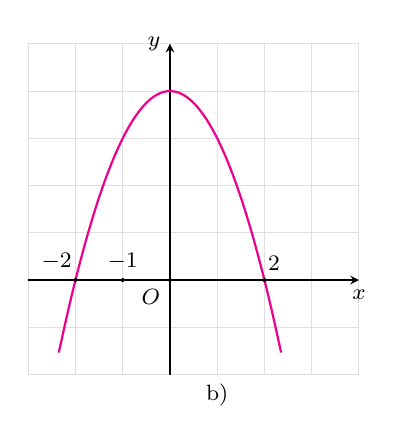
\begin{tikzpicture}[scale=.6, font=\footnotesize, line join=round, line cap=round,>=stealth]
		\draw[gray!50,opacity=.5](-3,-2)grid(4,5);
		\draw[->](-3,0)--(0,0)node[below left]{$O$}--(4,0)node[below]{$x$};
		\draw[->](0,-2)--(0,5)node[left]{$y$};
		\draw[smooth,domain=-2.35:2.35,thick, magenta]plot(\x,{-(\x)^2+4});
		\draw (1,-2)node[below]{b)};
		\draw(-2.4,0)node[above]{$-2$};
		\draw(-1,0)node[above]{$-1$};
		\draw(2.2,0)node[above]{$2$};
		\foreach \x in {-2,-1,0,2}\draw[fill](\x,0)circle(1pt);
	\end{tikzpicture}
	\item 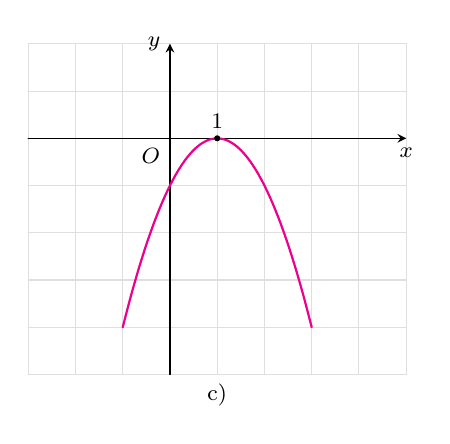
\begin{tikzpicture}[scale=.6, font=\footnotesize, line join=round, line cap=round,>=stealth]
		\draw[gray!50,opacity=.5](-3,-5)grid(5,2);
		\draw[->](-3,0)--(0,0)node[below left]{$O$}--(5,0)node[below]{$x$};
		\draw[->](0,-5)--(0,2)node[left]{$y$};
		\draw[smooth,domain=-1:3,thick, magenta]plot(\x,{-(\x-1)^2});
		\draw (1,-5)node[below]{c)};
		\draw(1,0)node[above]{$1$};
		\foreach \x in {1}\draw[fill](\x,0)circle(1.5pt);
	\end{tikzpicture}
	\end{enumerate}
	\loigiai{
\begin{enumerate}
	\item Phần đồ thị hàm số $f(x)$ nằm trên trục $Ox$ ứng với $x\in (-\infty;-1)\cup (2;+\infty)$.\\
	Vậy tập nghiệm của bất phương trình $f(x)>0$ là $(-\infty;-1)\cup (2;+\infty)$.
	\item Phần đồ thị hàm số $f(x)$ nằm trên trục $Ox$ ứng với $x\in (-2;2)$.\\
	Vậy tập nghiệm của bất phương trình $f(x)>0$ là $(-2;2)$.
	\item Đồ thị hàm số $f(x)$ nằm hoàn toàn bên dưới trục $Ox$, do đó bất phương trình $f(x)>0$ vô nghiệm.
\end{enumerate}
	}
\end{vd}

\begin{vd}%[Dự án đề cương 3 Khối NH25-26- Đợt 1- Nguyễn Cường]
	Tìm các giá trị của tham số $m$ để 
	\begin{multicols}{2}
		\begin{enumerate}
			\item $x^2-2x+m \ge 0,\, \forall x\in  \mathbb{R}$.
			\item $x^2 -2mx+4- 3m>0,\, \forall x\in  \mathbb{R}$. 
			\item $-x^2 -2(2m-1) x+1-2m \le 0,\, \forall x\in  \mathbb{R}$. 
			\item $-2x^2+2(m-2)x+m-2<0,\, \forall x\in  \mathbb{R} $. 
		\end{enumerate}
	\end{multicols}
	\loigiai{
		\begin{enumerate}
			\item  Ta có $\Delta'=(-1)^2-m=1-m$.\\			
			Khi đó, $x^2-2x+m \ge 0,\, \forall x\in  \mathbb{R}\Leftrightarrow\Delta'\le 0\Leftrightarrow 1-m\le 0\Leftrightarrow m\ge 1$.
			\item Ta có $\Delta '= b'^2-ac=m^2+3m-4$.\\
			Khi đó $x^2 -2mx+4- 3m>0,\, \forall x\in  \mathbb{R}\Leftrightarrow \heva{& a> 0\\& \Delta ' <0 } \Leftrightarrow \heva{& 1>0~\text{ (luôn đúng)}\\& m^2+3m -4 <0} \Leftrightarrow m^2+3m -4 <0$.\\
			Bảng xét dấu
			\begin{center}
				
\begin{tikzpicture}
					\tkzTabInit
					[lgt=2.5,espcl=2] % tùy chọn
					{$m $/1, $m^2+3m -4 $/1.3} % cột 1
					{$-\infty $,$-4$,$1$,$+ \infty $} % hàng 1 cột 2
					\tkzTabLine{,+ , z ,-, z ,+, } % hàng 2 cột 2
				\end{tikzpicture}
			\end{center}
			Dựa vào bảng xét dấu ta thấy $m \in (-4;1)$ thoả mãn yêu cầu bài toán.
			\item  Ta có $\Delta '=b'^2-ac=(2m-1)^2+(1-2m)=4m^2 -6m +2. $\\
			Khi đó $-x^2 -2(2m-1) x+1-2m \le 0,\, \forall x\in  \mathbb{R}\Leftrightarrow \heva{&a <0 \\& \Delta ' \le 0} \Leftrightarrow \heva{&-1<0 ~\text{ (luôn đúng)} \\& 4m^2-6m+2 \le 0} \Leftrightarrow 4m^2-6m+2 \le 0$.\\
			Bảng xét dấu
			\begin{center}
				
\begin{tikzpicture}
					\tkzTabInit
					[lgt=3 ,espcl=2] % tùy chọn
					{$m$/1, $4m^2 -6m +2  $/1.3} % cột 1
					{$-\infty $,$\dfrac{1}{2}$,$1$,$+ \infty $} % hàng 1 cột 2
					\tkzTabLine{,+ , z ,-, z ,+, } % hàng 2 cột 2
				\end{tikzpicture}
			\end{center}
			Dựa vào bảng xét dấu ta thấy $m \in \left[ \dfrac{1}{2};1\right]$ thoả mãn yêu cầu bài toán.
			\item Ta có $\Delta'=b'^2-ac=(m-2)^2+2(m-2)=m^2-2m$.\\
			Khi đó $-2x^2+2(m-2)x+m-2<0,\, \forall x\in  \mathbb{R}\Leftrightarrow \heva{&a <0 \\& \Delta ' \le 0} \Leftrightarrow \heva{&-2<0 ~\text{ (luôn đúng)} \\& m^2-2m<0} \Leftrightarrow m^2-2m<0$.\\
			Bảng xét dấu
			\begin{center}
				
\begin{tikzpicture}
					\tkzTabInit
					[lgt=3 ,espcl=2] % tùy chọn
					{$m$/.8, $m^2-2m$/1} % cột 1
					{$-\infty $,$0$,$2$,$+ \infty $} % hàng 1 cột 2
					\tkzTabLine{,+ , z ,-, z ,+, } % hàng 2 cột 2
				\end{tikzpicture}
			\end{center}
			Dựa vào bảng xét dấu ta thấy $m \in (0;2)$ thoả mãn yêu cầu bài toán.
%			Khi đó,
%			{\allowdisplaybreaks
%				\begin{eqnarray*}
%					&&f(x)=-2x^2+2(m-2)x+m-2\le 0,\forall x\in\mathbb{R} \\
%					&\Leftrightarrow & \Delta' =(m-2)^2+2\cdot(m-2)<0\\
%					&\Leftrightarrow & m(m-2)<0\\
%					&\Leftrightarrow & 0<m<2.
%			\end{eqnarray*}}
%			Vậy, giá trị cần tìm của $m$ là $0<m<2$.
		\end{enumerate}
	}
\end{vd}
\begin{dang}{Bài toán thực tế}
	Bài toán thực tế.
\end{dang}
\begin{vd}%[Dự án đề cương 3 Khối NH25-26- Đợt 1- Nguyễn Cường]
	Độ cao so với mặt đất của một quả bóng được ném lên theo phương thẳng đứng được mô tả bởi hàm số bậc hai $h(t)=-4{,}9 t^2+20t+1$, ở đó độ cao $h(t)$ tính bằng mét và thời gian $t$ tính bằng giây. Trong khoảng thời điểm nào trong quá trình bay của nó, quả bóng sẽ ở độ cao trên $5$ m so với mặt đất?
	\loigiai{
		Xét bất phương trình $-4{,}9 t^2+20t+1>5\Leftrightarrow-4{,}9 t^2+20t-4>0$.\\
		Nghiệm của phương trình
		$-4{,}9 t^2+20t-4=0$ là $t \approx 0{,}21;t \approx 3{,}87$.\\
		Do đó, nghiệm của bất phương trình là $t \in(0{,}21;3{,}87)$.\\
		Vậy khoảng thời điểm $t \in(0{,}21;3{,}87)$ giây trong quá trình bay của quả bóng thì nó sẽ ở độ cao trên $5$\,m so với mặt đất.
		}
\end{vd}

\begin{vd}%[Dự án đề cương 3 Khối NH25-26- Đợt 1- Nguyễn Cường]
	Một vật được ném theo phương thẳng đứng xuống dưới từ độ cao $320 \mathrm{~m}$ với vận tốc ban đầu $v_{Q}=20 \mathrm{~m} / \mathrm{s}$. Hỏi sau ít nhất bao nhiêu giây, vật đó cách mặt đất không quá $100 \mathrm{~m}$ ? Giả thiết rằng sức cản của không khí là không đáng kể.
	\loigiai{
		Độ cao của vật so với mặt đất được cho bởi công thức $
		h(t)=h_{0}+v_{0} t-\dfrac{1}{2} g t^2=320+20t-4{,}9 t^2(\mathrm{~m})$.\\
		Vật cách mặt đất không quá $100$\,m khi và chỉ khi $h(t) \le 100$.\\
		Nghĩa là $-4{,}9 t^2+20t+320 \le 100$ hay tương đương $4{,}9 t^2-20t-220 \ge 0$.\\
		Giải bất phương trình này và chú ý đến điều kiện $t>0$ ta được: $t \ge \dfrac{10+\sqrt{1178}}{4{,}9} \approx 9{,}05(\mathrm{~s})$.
	}
\end{vd}

\begin{vd}%[Dự án đề cương 3 Khối NH25-26- Đợt 1- Nguyễn Cường]
	\immini{Một tình huống trong huấn luyện pháo binh được mô tả như sau: Trong mặt phẳng tọa độ $Oxy$, khẩu đại bác được biểu thị bằng điểm $O(0; 0)$ và bia mục tiêu được biểu thị bằng đoạn thẳng $MN$ với $M(2100; 25)$ và $N(2100; 15)$ (Hình 29). Xạ thủ cần xác định parabol $y=-a^2x^2+10ax$ $(a>0)$ mô tả quỹ đạo chuyển động của viên đạn sao cho viên đạn bắn ra từ khẩu đại bác phải chạm vào bia mục tiêu. Tìm giá trị lớn nhất của $a$ để xạ thủ đạt được mục đích trên.
	}{\begin{tikzpicture}[scale=1, font=\footnotesize, line join=round, line cap=round,>=stealth]
			\def\a{-.25} \def\b{1} \def\c{0} % Hệ số
			\def\xt{-1} \def\xp{6} \def\yt{3} \def\yd{-1} % x_trái, x_phải, y_trên, y_dưới (giới hạn)
			\draw[->] (\xt,0)--(\xp,0) node [below]{$x$};
			\draw[->] (0,\yd)--(0,\yt) node [left]{$y$};
			\node at (0,0) [below left]{$O$};
			\clip (\xt-0.1,\yd+0.1) rectangle (\xp-0.1,\yt-0.1);
			\draw[smooth,samples=300,domain=0:4] plot(\x,{\a*(\x)^2+\b*(\x)+\c});
			\draw[fill=black] (3,0) node[shift={(-90:.4)}]{$2100$} circle(1pt);
			\draw[fill=black] (3,1) node[shift={(90:.4)}]{$M$} circle(1pt);
			\draw[fill=black] (3,.5) node[shift={(180:.3)}]{$N$} circle(1pt);
			\draw[line width=2pt] (3,1)--(3,.5);
			\draw (2,1) node[shift={(90:1)}]{$y=-a^2x^2+10ax$};
			\draw (2,-1) node[shift={(-90:.4)}]{Hình 29};
			
	\end{tikzpicture}}
	\loigiai
	{
		Tại vị trí $x=2\,100$, độ cao của viên đạn là
		\[y=-a^2\cdot 2\,100^2+10a\cdot 2\,100=-4\,410\,000a^2+21\,000a.\]
		Viên đạn chạm được vào bia mục tiêu khi và chỉ khi $a$ thoả mãn các bất phương trình sau
		\allowdisplaybreaks
		\begin{align*}
			&2100\le\dfrac{10}{a} \quad \quad (1); \\
			&-4410000a^2+21000a\le 25  \quad \quad (2);\\
			&-4410000a^2+21000a\ge 15.
		\end{align*}
		\begin{itemize}
			\item $(1\Leftrightarrow\dfrac{1}{a}\ge 210\Leftrightarrow a\le\dfrac{1}{210}$. Vì $a>0$ nên $a\in\left(0;\dfrac{1}{210}\right]$.
			\item $2) \Leftrightarrow 4410000a^2-21000a+25\ge 0 \Leftrightarrow(2100a-5)^2\ge 0$. Bất phương trình này đúng $\forall a>0$.
			\item \allowdisplaybreaks
			\begin{eqnarray*}
					-4410000a^2+21000a\ge 15&\Leftrightarrow& 4410000a^2-21000a+15\le 0\\
					&\Leftrightarrow&\dfrac{1}{420}-\dfrac{\sqrt{10}}{2100}\le a\le\dfrac{1}{420}+\dfrac{\sqrt{10}}{2100}\\
				&\Leftrightarrow& a\in\left[\dfrac{1}{420}-\dfrac{\sqrt{10}}{2100};\dfrac{1}{420}+\dfrac{\sqrt{10}}{2100}\right].
			\end{eqnarray*}
		\end{itemize}
		Do $\dfrac{1}{420}-\dfrac{\sqrt{10}}{2100}>0$ và $\dfrac{1}{420}+\dfrac{\sqrt{10}}{2100}<\dfrac{1}{210}$ nên
		\[\left(0;\dfrac{1}{210}\right]\cap\left[\dfrac{1}{420}-\dfrac{\sqrt{10}}{2100};\dfrac{1}{420}+\dfrac{\sqrt{10}}{2100}\right]=\left[\dfrac{1}{420}-\dfrac{\sqrt{10}}{2100};\dfrac{1}{420}+\dfrac{\sqrt{10}}{2100}\right].\]
		Vì thế, viên đạn chạm được vào bia mục tiêu khi và chỉ khi
		\[a\in\left[\dfrac{1}{420}-\dfrac{\sqrt{10}}{2100};\dfrac{1}{420}+\dfrac{\sqrt{10}}{2100}\right].\]
		Vậy giá trị lớn nhất của $a$ là $\dfrac{1}{420}+\dfrac{\sqrt{10}}{2100}$.
	}
\end{vd}
%-----------------------------------------------------------------------------
\subsection{Bài tập rèn luyện}
\ind{PHẦN I.} \inden{Câu trắc nghiệm nhiều phương án lựa chọn. Mỗi câu hỏi học sinh chỉ chọn một phương án.}\\
\setcounter{ex}{0}
\Opensolutionfile{ans}[ans/0D7-Bai2-TN]%--Đặt tên 0D7-Bai2-Dang1-TN
\begin{ex}[THPT Lý Tự Trọng - Khánh Hoà]%[0D7N2-1]%[Dự án đề cương 3 Khối NH25-26- Đợt 1- Nguyễn Cường]
	Tập nghiệm của bất phương trình $x^2-4 x+3>0$ là
	\choice
	{$(1 ; 3)$}
	{\True $(-\infty ; 1) \cup(3 ;+\infty)$}
	{$(-\infty ; 1] \cup [3 ;+\infty)$}
	{$[1;3]$}
	\loigiai{Xét $x^2-4 x+3=0\Leftrightarrow \hoac{&x=1\\&x=3.}$\\
		Bảng xét dấu
		\begin{center}
			\begin{tikzpicture}
				\tkzTabInit[nocadre=false,lgt=4,espcl=2.5,deltacl=0.6]
				{$x$ /0.6, $x^2-4x+3$ /1}
				{$-\infty$,$1$,$3$,$+\infty$}
				\tkzTabLine{,+,0,-,0,+,}
				\begin{scope}[on background layer]\path[white]node{MDD-904};\end{scope}
			\end{tikzpicture}
		\end{center}
		Do đó $S=(-\infty ; 1) \cup(3 ;+\infty)$.
	}
\end{ex}

\begin{ex}[THPT Tân Bình - Tp HCM]%[0D7N2-1]%[Dự án đề cương 3 Khối NH25-26- Đợt 1- Nguyễn Cường]
	Giá trị $x_0$ nào sau đây là nghiệm của bất phương trình $x^2+8x+15< 0$?
	\choice
	{$x_0=-3$}
	{\True $x_0=-4$}
	{$x_0=1$}
	{$x_0=-6$}
	\loigiai{
		Thay $x_0=-4$ vào bất phương trình $x^2+8x+15< 0$ ta được $16-32+15<0$ (đúng) nên $x_0=-4$ là nghiệm của bất phương trình đã cho.
	}
\end{ex}

\begin{ex}[THPT Tân Bình - Tp HCM]%[0D7N2-1]%[Dự án đề cương 3 Khối NH25-26- Đợt 1- Nguyễn Cường]
	Bất phương trình nào dưới đây là bất phương trình bậc hai một ẩn?
	\choice
	{$2x^2-3x^3+1\leq 0$}
	{\True $9-x^2> 0$}
	{$1-x \leq 0$}
	{$x\left(x^2-3x+2\right) > 0$}
	\loigiai{
		Bất phương trình bậc hai 1 ẩn số là $9-x^2> 0$.
	}
\end{ex}

\begin{ex}[THPT Trần Phú-Tp.HCM]%[0D7N2-2]%[Dự án đề cương 3 Khối NH25-26- Đợt 1- Nguyễn Cường]
	Hàm số $y=f(x)$ có đồ thị như hình vẽ.
	\begin{center} 
		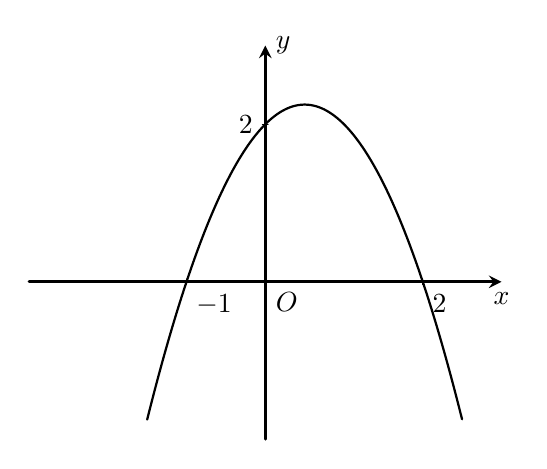
\begin{tikzpicture}[line join = round, line cap = round,>=stealth,thick,x = 1cm,y = 1cm] 
			%Vẽ hệ trục Oxy 
			\draw[->,line width = 1pt] (-3,0)--(0,0) node[below right]{$O$}--(3,0) node[below]{$x$}; 
			\draw[->,line width = 1pt] (0,-2.0)--(0,3) node[right]{$y$}; 
			%Vẽ các điểm gióng 
			\foreach \x in {-1,2} \draw[thin] (\x,1pt)--(\x,-1pt) node [below right] {$\x$}; 
			\foreach \y in {2} \draw[thin] (1pt,\y)--(-1pt,\y) node [left] {$\y$}; 	\draw[samples=200,domain=-1.5:2.5,smooth] plot (\x, {-(\x)^2 +(\x)+2}); 
		\end{tikzpicture}
	\end{center}
	Tập nghiệm $S$ của bất phương trình $f(x)>0$ là
	\choice
	{$S=\left(-\infty; -1] \cup[2; +\infty\right)$}
	{\True $S=\left(-1;2\right)$}
	{$S=\left(0;2\right]$}
	{$S=\left(-\infty; -1) \cup(2; +\infty\right)$}
	\loigiai{
		Nhìn vào đồ thị, ta thấy $f(x)>0$ khi và chỉ khi $x \in \left(-1;2\right)$.
	}
\end{ex}

\begin{ex}[THPT Mạc Đĩnh Chi - Tp.HCM]%[0D7N2-1]%[Dự án đề cương 3 Khối NH25-26- Đợt 1- Nguyễn Cường]
	Tập nghiệm $S$ của bất phương trình $x^2-6 x+8<0$ là
	\choice
	{$S=[2 ; 4]$}{\True $S=(2 ; 4)$}{$S=[2 ; 4)$}{$S=(2 ; 4]$}
	\loigiai{
		Ta có $x^2-6 x+8<0 \Leftrightarrow 2<x<4$.\\
		Vậy tập nghiệm là $S=(2;4)$.
	}
\end{ex}

\begin{ex}[THPT Nguyễn Thái Bình-TPHCM]%[0D7N2-1]%[Dự án đề cương 3 Khối NH25-26- Đợt 1- Nguyễn Cường]
	Bất phương trình nào dưới đây \textbf{không} phải là bất phương trình bậc hai một ẩn $x$?
	\choice
	{ $-x^2-1 \ge 0$}
	{\True $x+2>0$}
	{ $-2x^2+x-3<0$}
	{$3x^2-2x-1 \le 0$}
	\loigiai{
		Bất phương trình $x+2>0$ không phải là bất phương trình bậc hai một ẩn.
	}
\end{ex}
\begin{ex}[THPT Ngọc Tảo- Hà Nội]%[0D7N2-1]%[Dự án đề cương 3 Khối NH25-26- Đợt 1- Nguyễn Cường]
	Tập nghiệm của bất phương trình $-x^2+3x+18>0$ là
	\choice
	{$[-3;6]$}
	{\True $(-3;6)$}
	{$(-\infty;-3)\cup (6;+\infty)$}
	{$(-\infty;-3]\cup [6;+\infty)$}
	\loigiai
	{Tam thức bậc hai $f(x)=-x^2+3x+18$ có hai nghiệm là $-3$ và $6$.\\
		Do hệ số $a=-1<0$ nên ta có dấu của $f(x)$ như sau:
		\begin{center}
			\begin{tikzpicture} [scale=0.5, font=\footnotesize, line cap = round, line join = roud, >=stealth]
				\draw[->] (-6,0)--(9,0);
				\path (-3,0) node {|} node[below = 6pt]{$-3$} (6,0) node {|} node[below = 6pt]{$6$};
				\path (-4.5,0) node[below = 6pt]{$-$} (7.5,0) node[below = 6pt]{$-$};
				\path (1.5,0) node[above = 6pt]{$+$};
			\end{tikzpicture}
		\end{center}
		Vậy tập nghiệm của bất phương trình $-x^2+3x+18>0$ là khoảng $(-3;6)$.}
\end{ex}

\begin{ex}%[0D7N2-1]%[Dự án đề cương 3 Khối NH25-26- Đợt 1- Nguyễn Cường]
	Nghiệm của bất phương trình $x^2-8x+15 \leq 0$
	\choice
	{\True $x \in \left[3;5\right]$}
	{$x \in \left(3;5\right)$}
	{$x \in \left(-\infty;3\right] \cup \left[5;+\infty\right)$}
	{$x \in \left(-\infty;3\right) \cup \left(5;+\infty\right)$}
	\loigiai{
		Ta có $x^2-8x+15 \leq 0 \Leftrightarrow (x-3)(x-5)\leq 0$ suy ra bảng xét dấu dưới đây
		\begin{center}
			
\begin{tikzpicture}
				\tkzTabInit%[nocadre,lgt=1.2,espcl=2]
				{$x$/0.7,$f(x)$/0.7}{$-\infty$,$3$,$5$,$+\infty$}
				\tkzTabLine{,-,0,+,0,-,}  
			\end{tikzpicture}
		\end{center}
		Dựa vào bảng xét dấu dễ dàng suy ra được kết quả là $x \in \left[3;5\right]$.
	}
\end{ex}

\begin{ex}[THPT Tân Bình - Tp HCM]%[0D7H2-2]%[Dự án đề cương 3 Khối NH25-26- Đợt 1- Nguyễn Cường]
	Cho tam thức bậc hai $f(x)$ có bảng xét dấu như sau
	\begin{center}
		
\begin{tikzpicture}
			\tkzTabInit%[nocadre,lgt=1.2,espcl=2]
			{$x$/0.7,$f(x)$/0.7}{$-\infty$,$-1$,$5$,$+\infty$}
			\tkzTabLine{,-,0,+,0,-,}	 
		\end{tikzpicture}
	\end{center}
	Tập nghiệm của bất phương trình $f(x) \geq 0$ là
	\choice
	{$S=[-5; 1]$}
	{$S=(-\infty;-1] \cup[5;+\infty)$}
	{\True $S=[-1; 5]$}
	{$S=(-\infty;-5] \cup[1;+\infty)$}
	\loigiai{
		Dựa vào bảng xét dấu, ta thấy $f(x) \geq 0 \Leftrightarrow  -1 \leq x \leq 5$ nên tập nghiệm của bất phương trình đã cho là $S=[-1; 5]$.
	}
\end{ex}

\begin{ex}[THPT Trần Phú-Tp.HCM]%[0D7N2-2]%[Dự án đề cương 3 Khối NH25-26- Đợt 1- Nguyễn Cường]
\immini{Hàm số $y=f(x)$ có đồ thị như hình vẽ. Tập nghiệm $S$ của bất phương trình $f(x)>0$ là
	\choice
	{$S=\left(-\infty; -1] \cup[2; +\infty\right)$}
	{\True $S=\left(-1;2\right)$}
	{$S=\left(0;2\right]$}
	{$S=\left(-\infty; -1) \cup(2; +\infty\right)$}
}
{
	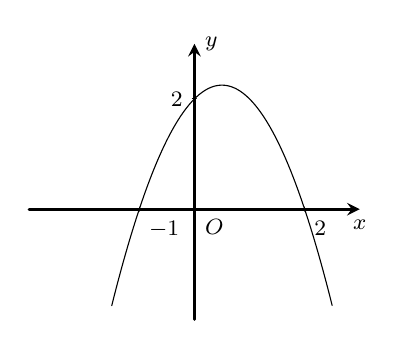
\begin{tikzpicture}[line join = round, line cap = round,>=stealth,font=\footnotesize,scale=.7] 
	%Vẽ hệ trục Oxy 
	\draw[->,line width = 1pt] (-3,0)--(0,0) node[below right]{$O$}--(3,0) node[below]{$x$}; 
	\draw[->,line width = 1pt] (0,-2.0)--(0,3) node[right]{$y$}; 
	%Vẽ các điểm gióng 
	\foreach \x in {-1,2} \draw[thin] (\x,1pt)--(\x,-1pt) node [below right] {$\x$}; 
	\foreach \y in {2} \draw[thin] (1pt,\y)--(-1pt,\y) node [left] {$\y$}; 	\draw[samples=200,domain=-1.5:2.5,smooth] plot (\x, {-(\x)^2 +(\x)+2}); 
\end{tikzpicture}
}
	\loigiai{
		Nhìn vào đồ thị, ta thấy $f(x)>0$ khi và chỉ khi $x \in \left(-1;2\right)$.
	}
\end{ex}

\begin{ex}[THPT Nguyễn Thái Bình-TPHCM]%[0D7H2-2]%[Dự án đề cương 3 Khối NH25-26- Đợt 1- Nguyễn Cường]
	\immini
	{
		Cho đồ thị hàm số bậc hai $f(x)=ax^2+bx+c\ (a \ne 0)$ như hình vẽ. Tập nghiệm $S$ của bất phương trình $f(x)>0$ là
		\choice{\True $S=(-1;3)$}{$S=(-1;4)$}{$S=(0;4)$}{$S=(1;4)$}
	}
	{
		\begin{tikzpicture}[>=stealth,x=1.0cm,y=1.0cm,scale=0.7,line cap=round,line join=round]
			\draw[->] (-2,0) -- (4,0) node[below] { $x$};
			\draw[->] (0,-1) -- (0,5) node[right] { $y$};
			\draw[dashed,thin] (0,4)--(1,4)--(1,0);
			\draw (0,4) node[left]{$4$} 
			(1,0) node[below]{$1$};
			\draw[domain=-1.1:3.1,samples=150] plot (\x,{-(\x)^2+2*(\x)+3});
			\draw[fill=black] (-1,0) circle (1pt) node[above left]{$-1$} (3,0) circle (1pt) node[above right] {$3$};
		\end{tikzpicture}
	}
	\loigiai{
		Dựa vào đồ thị hàm số, tập nghiệm $S$ của bất phương trình $f(x)>0$ là $S=(-1;3)$.
	}
\end{ex}

\begin{ex}[THPT Nguyễn Thái Bình-TPHCM]%[0D7H2-2]%[Dự án đề cương 3 Khối NH25-26- Đợt 1- Nguyễn Cường]
	\immini
	{
		Cho hàm số bậc hai $y=f(x)$ có đồ thị như hình vẽ. Khẳng định nào dưới đây đúng?
		\choice{$f(x)>0, \forall x \in(-\infty ;-4] \cup[0 ;+\infty)$}{$f(x)<0, \forall x \in(-\infty ;-4] \cup[0 ;+\infty)$}{$f(x) \ge 0, \forall x \in[-4 ; 0]$}{\True $f(x) \le 0, \forall x \in[-4 ; 0]$}
	}
	{
		\begin{tikzpicture}[scale=0.75, font=\footnotesize, line join=round, line cap=round, >=stealth]
			\draw[->] (-5.5,0)--(1.5,0) node[below left] {$x$};
			\draw[->] (0,-3)--(0,1.5) node[below right] {$y$};
			\draw (0,0) node [above left] {$O$};
			\foreach \x in {-4}
			\draw[] (\x,1pt)--(\x,-1pt) node [below left] {$\x$};
			\foreach \y in {-2}
			\draw[] (1pt,\y)--(-1pt,\y) node [below right] {$\y$};
			\draw (-2,0) node[above]{$-2$};
			\begin{scope}
				%\clip (-1.5,-1.5) rectangle (3.5,2.5);
				\draw[samples=200,domain=-4.3:0.3,smooth,variable=\x] plot (\x,{0.5*(\x)^2+2*(\x)});
			\end{scope}
			\draw[dashed] (-2,0)|-(0,-2);
		\end{tikzpicture}
	}
	\loigiai{
		Dựa vào đồ thị ta có  $f(x) \le 0, \forall x \in[-4 ; 0]$.
	}
\end{ex}
\begin{ex}%[0D7N2-1]%[Dự án đề cương 3 Khối NH25-26- Đợt 1- Nguyễn Cường]
Bất phương trình $ax^2+bx+c\leq 0$ với $a\ne 0$ luôn đúng khi và chỉ khi 
\choice
{$\heva{& a>0\\& \Delta\leq 0}$}
{\True $\heva{& a<0\\& \Delta\leq 0}$}
{$\heva{& a>0\\& \Delta\geq 0}$}
{$\heva{& a<0\\& \Delta\geq 0}$}
\loigiai{
	Ta có $f(x)\leq 0$, $\forall x\in\mathbb{R}$ $\Leftrightarrow \heva{& a<0\\& \Delta\leq 0.}$
}
\end{ex}
\begin{ex}[THPT Nguyễn Thái Bình, HCM, 2024]%[0D7N2-1]%[Dự án đề cương 3 Khối NH25-26- Đợt 1- Nguyễn Cường]
	Tập nghiệm $S$ của bất phương trình $-x^2-2x+8>0$ là
	\choice
	{$S=(-2; 4)$}
	{$S=(-\infty;-4)\cup(2;+\infty)$}
	{$S=\{-4; 2\}$}
	{\True $S=(-4; 2)$}
	\loigiai{
		Ta có $-x^2-2x+8>0\Leftrightarrow x\in (-4;2)$.\\
		Vậy tập nghiệm của bất phương trình đã cho là $S=(-4; 2)$.
	}
\end{ex}

\begin{ex}[THPT Lương Ngọc Quyến - Thái Nguyên]%[0D7N2-1]%[Dự án đề cương 3 Khối NH25-26- Đợt 1- Nguyễn Cường]
	Tập nghiệm của bất phương trình $-x^2+5x-4<0$ là
	\choice
	{$(-\infty;1]\cup [4;+\infty)$}
	{$(1;4)$}
	{$[1;4]$}
	{\True $(-\infty;1)\cup (4;+\infty)$}
	\loigiai{
		Ta có $-x^2+5x-4<0\Leftrightarrow \hoac{&x<1\\&x>4.}$\\
		Tập nghiệm của bất phương trình là $S=(-\infty;1)\cup (4;+\infty)$.
	}
\end{ex}

\begin{ex}[THPT Triệu Sơn 4-Thanh Hóa]%[0D7H2-6]%[Dự án đề cương 3 Khối NH25-26- Đợt 1- Nguyễn Cường]
	Bất phương trình $-x^2+4x-m>0$ vô nghiệm khi
	\choice
	{$m>4$}
	{$m \leq 4$}
	{\True $m \geq 4$}
	{$m<4$}
	\loigiai{
		Bất phương trình $-x^2+4x-m>0$ vô nghiệm khi và chỉ khi $-x^2+4x-m \leq 0, \forall x \in \mathbb{R}$.
		\[\begin{aligned}
			&-x^2+4x-m \leq 0, \forall x \in \mathbb{R}\\
			\Leftrightarrow & \heva{& a < 0\\& \Delta \leq 0}\\
			\Leftrightarrow & \heva{& -1<0 \\& 16-4m \leq 0}\\
			\Leftrightarrow & m \geq 4.\\
		\end{aligned}\]
	}
\end{ex}

\begin{ex}%[0D7H2-6]%[Dự án đề cương 3 Khối NH25-26- Đợt 1- Nguyễn Cường]
	Với giá trị nào của $m$ thì bất phương trình $-x^2-x+m\geq0$ vô nghiệm?
	\choice
	{$m \geq-\dfrac{1}{4}$}
	{$m >-\dfrac{1}{4}$}
	{$m \leq-\dfrac{1}{4}$}
	{\True $m <-\dfrac{1}{4}$}
	\loigiai{
		Bất phương trình $-x^2-x+m\geq0$ vô nghiệm, khi và chỉ khi $-x^2-x+m<0, \forall x \in \mathbb{R}$.\\
		Ta có $-x^2-x+m<0, \forall x \in \mathbb{R} \Leftrightarrow 
		\heva{&a<0\\&\Delta<0}
		\Leftrightarrow\heva{&-1<0\\&{{\left(-1\right)}^2}-4\cdot \left(-1\right)\cdot m<0}
		\Leftrightarrow m<-\dfrac{1}{4}$.
	}
\end{ex}

\begin{ex}%[0D7H2-6]%[Dự án đề cương 3 Khối NH25-26- Đợt 1- Nguyễn Cường]
	Tìm tất cả các giá trị của $m$ để bất phương trình $x^2-(m+2)x+5 m+1 \ge 0$ với mọi $x$.
	\choice
	{$m>16$}
	{\True $0\leq m\leq16$}
	{$m<16$}
	{$0<m<16$}
	\loigiai{
		Tam thức $f(x)=x^2-(m+2)x+5 m+1$ không âm với mọi $x$ thì $\heva{&a>0\\&\Delta\leq0}\Leftrightarrow\left(m+2\right)^2-4\cdot\left(5m+1\right)\leq0\Leftrightarrow m^2-16m\leq 0\Leftrightarrow 0\leq m\leq16$.
	}
\end{ex}

\begin{ex}[THPT Nguyễn Thượng Hiền-Tp HCM]%[0D7H2-6]%[Dự án đề cương 3 Khối NH25-26- Đợt 1- Nguyễn Cường]
	Tìm tất cả các giá trị của $m$ để bất phương trình $x^2-x+m \leq 0$ vô nghiệm.
	\choice
	{$m > 1$}
	{$m < \dfrac{1}{4}$}
	{$m < 1$}
	{\True $m > \dfrac{1}{4}$}
	\loigiai{
		Bất phương trình $x^2-x+m \leq 0$ vô nghiệm tương đương
		\begin{eqnarray*}
			x^2-x+m > 0,\;\forall x\in\mathbb{R} &\Leftrightarrow& \heva{&a>0\\&\Delta<0} \\
			&\Leftrightarrow& (-1)^2-4m<0\\
			&\Leftrightarrow& m>\dfrac{1}{4}.
		\end{eqnarray*}
	}
\end{ex}

\begin{ex}[ THPT Nguyễn Khuyến-Bình Dương]%[0D7H2-6]%[Dự án đề cương 3 Khối NH25-26- Đợt 1- Nguyễn Cường]
	Có bao nhiêu giá trị nguyên của $m$ để bất phương trình $x^2+2mx+4\ge0$ có tập nghiệm là $\mathbb{R}$?
	\choice
	{$3$}
	{$4$}
	{\True $5$}
	{$6$}
	\loigiai{Bất phương trình đã cho có tập nghiệm là $\mathbb{R}$ khi và chỉ khi $$\heva{&a=1>0\\ 
			&\Delta'\le0}\Leftrightarrow m^2-4\le0\Leftrightarrow-2\le m\le2.$$ Suy ra $m\in\{-2;-1;0;1;2\}$.\\
		Vậy có $5$ giá trị của $m$ thỏa yêu cầu đề bài.
	}
\end{ex}
\Closesolutionfile{ans}

\ind{PHẦN II.} \inden{Câu trắc nghiệm đúng sai. Trong mỗi ý a), b), c), d) ở mỗi câu, học sinh chọn đúng hoặc sai.}\\
\setcounter{ex}{0}
\Opensolutionfile{ans}[ans/0D7-Bai2-DS]%--Đặt tên 0D7-Bai2-DS


\begin{ex}%[0D7H2-2]%[Dự án đề cương 3 Khối NH25-26- Đợt 1- Nguyễn Cường]
	Cho hàm số $f(x)$ có đồ thị như hình vẽ bên
	\immini{
		\choiceTF
		{Tập nghiệm của bất phương trình $f(x) < 0$ là $\mathbb{R} \setminus(1; 3)$}
		{\True Tập nghiệm của bất phương trình $f(x) \geq 0$ là $S=[1; 3]$}
		{Nghiệm $x=1$ là một nghiệm của bất phương trình $f(x) > 0$}
		{Bất phương trình $f(x) < 2$ có tập nghiệm $S=\mathbb{R}$}
	}{
		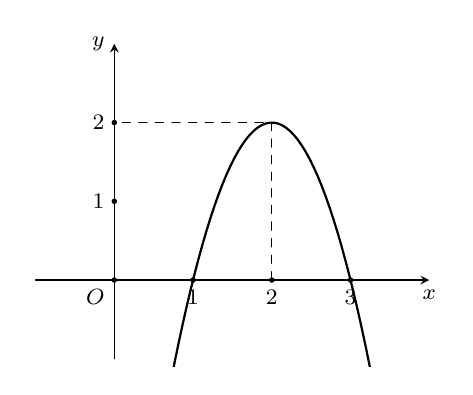
\begin{tikzpicture}[scale=1, font=\footnotesize, line join=round, line cap=round,>=stealth]
			%Gán số liệu.
			\def\xmin{-1};\def\ymin{-1};\def\xmax{4};\def\ymax{3};
			%Gán tọa độ.
			\coordinate (O) at (0,0);
			%Trục Oxy.
			\draw[->] (\xmin,0)--(\xmax,0) node[below]{$x$};
			\draw[->] (0,\ymin)--(0,\ymax) node[left]{$y$};
			\fill (O) node[below left]{$O$} circle(1pt);
			%Giới hạn đồ thị.
			\clip ({\xmin-0.1},{\ymin-0.1}) rectangle ({\xmax+0.1},{\ymax+0.1});
			\foreach \x in {1,2,3}{
				\fill (\x,0) node[below]{$\x$} circle(1pt);
			}
			\foreach \y in {1,2}{
				\fill (0,\y) node[left]{$\y$} circle(1pt);
			}
			%Vẽ đồ thị.
			\draw [dashed] (2,0)--(2,2)--(0,2);
			\draw[thick,samples=100] plot[domain=-1:4](\x,{-2*(\x)^2+8*\x-6});
		\end{tikzpicture}
	}
	\loigiai{
		\begin{itemchoice}
			\itemch Tập nghiệm của bất phương trình $f(x) < 0$ là $\mathbb{R} \setminus[1; 3]$.
			\itemch Tập nghiệm của bất phương trình $f(x) \geq 0$ là $S=[1; 3]$.
			\itemch Tập nghiệm của bất phương trình $f(x) > 0$ là $S=(1; 3)$ mà $x=1\notin(1; 3)$.
			\itemch Bất phương trình $f(x) < 2$ có tập nghiệm $S=\mathbb{R} \setminus\{2\}$.
		\end{itemchoice}
	}
\end{ex}
\begin{ex}[Sở Bắc Giang]%[0D7H2-1]%[Dự án đề cương 3 Khối NH25-26- Đợt 1- Nguyễn Cường]
	Cho hàm số $y=f(x)=-x^2+3x-2$.
	\choiceTF
	{\True Tập nghiệm của bất phương trình $f(x)\geq 0$ là $[1;2]$}
	{\True Phương trình $f(x)=0$ có hai nghiệm phân biệt}
	{Giá trị lớn nhất của hàm số $f(x)$ bằng $\dfrac{3}{2}$}
	{Có duy nhất một giá trị nguyên dương của $m$ để phương trình $f(x)=m$ có hai nghiệm phân biệt}
	\loigiai
	{	\begin{itemchoice}
			\itemch Ta có $-x^2+3x-2\geq 0 \Leftrightarrow 1\leq x\leq 2$.\\
			Vậy tập nghiệm của bất phương trình $-x^2+3x-2\geq 0$ là $[1;2]$. 
			\itemch $f(x)=0\Leftrightarrow -x^2+3x-2=0\Leftrightarrow \hoac{&x=1\\&x=2}$ nên phương trình có hai nghiệm phân biệt.
			\itemch Ta có $f(x)=\dfrac{1}{4}-\left(x-\dfrac{3}{2}\right)^2\leq \dfrac{1}{4}$, đẳng thức xảy ra khi và chỉ khi $x=\dfrac{3}{2}$.\\
			Do đó giá trị lớn nhất của hàm số bằng $f\left(\dfrac{3}{2}\right)=\dfrac{1}{4}$.
			\itemch  Ta có đồ thị của hàm số $y=f(x)$ như sau
			\begin{center}
				\begin{tikzpicture}[line join=round, line cap=round,>=stealth,xscale=1,yscale=1.2]
					\tikzset{every node/.style={scale=0.9}}
					\draw[->] (-2.1,0)--(4.1,0) node[below left] {$x$};
					\draw[->] (0,-2.9)--(0,1.1) node[below left] {$y$};
					\draw (0,0) node [below left] {$O$};
					\draw [dashed] (1.5,0)node[below]{$\tfrac{3}{2}$}--(1.5,0.25)--(0,.25)node[left]{$\tfrac{1}{4}$} (0,-2)node[left]{$-2$};
					\begin{scope}
						\clip (-2,-2.9) rectangle (4.5,2);
						\draw[samples=200,domain=-1:4,smooth,variable=\x] plot (\x,{-1*(\x)^2+3*(\x)+-2});
					\end{scope}
				\end{tikzpicture}
			\end{center}
			Từ đồ thị ta thấy phương trình $f(x)=m$ có hai nghiệm phân biệt khi và chỉ khi $m<\dfrac{1}{4}$ nên không có giá trị nguyên dương nào của $m$ thỏa mãn yêu cầu bài toán.
		\end{itemchoice}
		
	}
\end{ex}

\begin{ex}%[0D7V2-6]%[Dự án đề cương 3 Khối NH25-26- Đợt 1- Nguyễn Cường]
	Cho $f(x)=x^2-2(m+1)x+4$ ($m$ là tham số thực).
	\choiceTF
	{\True $f(x)$ là tam thức bậc hai với mọi giá trị của tham số $m$}
	{Khi $m=-\dfrac{1}{2}$ thì $f(x)<0, \forall x\in[-2; 3]$}
	{\True Khi $m=1$ thì hàm số $y=\sqrt{f(x)}$ có tập xác định là $\mathbb{R}$}
	{\True Có hai giá trị nguyên âm của tham số $m$ để $f(x)> 0$, $\forall x\in\mathbb{R}$}
	\loigiai{\begin{itemchoice}
			\itemch Vì $a=1\neq 0$ nên $f(x)=x^2-2(m+1)x+4$ là tam thức bậc hai với mọi giá trị của $m$.
			\itemch Với $m=-\dfrac{1}{2}$ ta có $f(x)=x^2-x+4$.\\
			Tam thức có hệ số $a=1>0$ và $\Delta=(-1)^2-4\cdot 1
			\cdot 4=-15<0$ nên $f(x)>0, \forall x\in\mathbb{R}$.
			\itemch Vì khi $m=1$ ta có $y=\sqrt{f(x)}=\sqrt{x^2-4x+4}$.\\
			Do $x^2-4x+4=(x+2)^2\geq 0, \forall x\in \mathbb{R}$ nên hàm số $y=\sqrt{f(x)}$ có tập xác định là $\mathbb{R}$.
			\itemch Vì $f(x)>0$, $\forall x\in\mathbb{R} \Leftrightarrow \Delta'<0\Leftrightarrow(m+1)^2-4< 0\Leftrightarrow-3<m<1$.\\
			Mà $m$ là số nguyên âm nên $\,m \in\{-2;-1\}$.\\
			Vậy có hai giá trị nguyên âm của tham số $m$ để $f(x)>0$, $\forall x \in\mathbb{R}$.
		\end{itemchoice}
	}
\end{ex}
\begin{ex}[THPT Dĩ An- Bình Dương]%[0D7H2-6]%[Dự án đề cương 3 Khối NH25-26- Đợt 1- Nguyễn Cường]
	Cho tam thức bậc hai $f(x)=x^2-2(2m-3)x+4m-3$ với $m$ là tham số thực.
	\choiceTF
	{\True Khi $m=1$ ta có tam thức bậc hai là $f(x)=x^2+2x+1$}
	{Biệt thức $\Delta $ của tam thức $f(x)$ là $\Delta =16m^2-48m+36$}
	{\True Khi $m=2$ thì tập nghiệm của bất phương trình $f(x)>0$ là $S=\mathbb{R}$}
	{\True Tam thức $f(x)$ luôn dương trên $\mathbb{R}$ khi $1<m<3$}
	\loigiai{\begin{itemchoice}
			\itemch Thế $m=1$ vào tam thức bậc hai ta được $f(x)=x^2+2x+1$.
			\itemch Ta có $a=1$, $b=-2(2m-3)$, $c=4m-3$.\\
			Suy ra 
			\begin{align*}
				\Delta&=4(2m-3)^2-4(4m-3)\\
				&=16m^2-48m+36-16m+12\\
				&=16m^2-64m+48.
			\end{align*}
			\itemch Khi $m=2$ thì $f(x)=x^2-2x+5>0 \Leftrightarrow x \in \mathbb{R}$.
			\itemch Ta có $a=1>0$. Khi đó,
			\[f(x)>0, \forall x\in \mathbb{R} \Leftrightarrow \heva{&a>0\\&\Delta <0}\Leftrightarrow \heva{&a=1>0 \text{ (đúng)}\\&16m^2-60m+48<0}\Leftrightarrow 1<m<3.\]
		\end{itemchoice}
	}
\end{ex}

\begin{ex}%[0D7V2-7]%[Dự án đề cương 3 Khối NH25-26- Đợt 1- Nguyễn Cường]
	Công ty A có $100$ cán bộ công nhân viên và muốn tổ chức cho toàn công ty đi Year End Party tại khu du lịch Tam Đảo, Vĩnh Phúc. Một công ty du lịch chào giá vé với công ty A như sau: 
	\begin{itemize}
		\item Với $40$ khách hàng đầu tiên có giá vé là $3$ triệu đồng/người.
		\item Có nhiều hơn $40$ khách hàng thì cứ thêm $1$ người giá vé sẽ giảm $15000$ đồng/người cho toàn bộ hành khách.
	\end{itemize}
	Gọi $x$ là số lượng cán bộ công nhân viên của công ty A thứ $41$ trở lên. Biết chi phí thực tế công ty du lịch dành cho mỗi khách hàng là $1{,}95$ triệu đồng.
	\choiceTF 
	{\True Giá vé còn lại sau khi thêm $x$ người là $3000-15x$ (nghìn đồng/người)}
	{Chi phí thực tế cho chuyến đi này là $1950(40-x)$ (nghìn đồng)}
	{Lợi nhuận của công ty du lịch đạt được biểu thị bằng công thức $T=15x^2-450x+42000$ (nghìn đồng)}
	{\True Số cán bộ công nhân viên công ty A đăng ký tối thiểu là $50$ người thì công ty du lịch đạt lợi nhuận tối thiểu $45$ triệu đồng}
	\loigiai{
		\begin{itemchoice}
			\itemch Vì cứ nhiều hơn $40$ người đăng ký thì cứ thêm $1$ người giá vé sẽ giảm $15000$ đồng/người cho toàn bộ hành khách nên thêm $x$ người giá vé còn $3000-15x$ (nghìn đồng/người).
			\itemch Chi phí thực tế cho chuyến đi là $1950(40+x)$ (nghìn đồng).
			\itemch Doanh thu của công ty du lịch là $(3000-15x)(40+x)$ (nghìn đồng). \\
			Lợi nhuận của công ty du lịch đạt được là 
			\allowdisplaybreaks
			\begin{eqnarray*}
				T &=& (3000-15x)(40+x)-1950(40+x)\\
				&=&-15x^2-600x+3000x+120000-1950x-78000\\
				&=&-15x^2+450x+42000\quad\text{(nghìn đồng)}
			\end{eqnarray*} 
			\itemch Để lợi nhuận công ty tối thiểu là $45$ triệu đồng thì $$T\ge45000\Leftrightarrow-15x^2+450x+42000\ge45000\Leftrightarrow-15x^2+450x-3000\ge0\Leftrightarrow10\le x\le20.$$ 
			Vậy số cán bộ công nhân viên công ty A đăng ký tối thiểu là $50$ người thì công ty du lịch đạt lợi nhuận tối thiểu $45$ triệu đồng.
	\end{itemchoice}
}
\end{ex}
\Closesolutionfile{ans}


\ind{PHẦN III.} \inden{Câu trắc nghiệm trả lời ngắn}\\
\setcounter{ex}{0}
\Opensolutionfile{ans}[ans/0D7-Bai2-TLN]%--Đặt tên 0D7-Bai2-DS

\begin{ex}[THPT Thực Hành Sư Phạm Tp.HCM]%[0D7H2-1]%[Dự án đề cương 3 Khối NH25-26- Đợt 1- Nguyễn Cường]
	Tập hợp tất cả các giá trị thực của tham số $m$ để $3 x^2+2(2 m-1) x+m+4>0$, $\forall x \in \mathbb{R}$ là $(a;b)$. Tính $b$.
	\shortans[]{$2{,}75$}
	\loigiai
	{
		Ta có
	\allowdisplaybreaks
	\begin{eqnarray*}
		3 x^2+2(2 m-1) x+m+4>0, \forall x \in \mathbb{R}&\Leftrightarrow& \heva{& a=3>0 \\ & \Delta'<0}\\ &\Leftrightarrow& 4 m^2-7 m-11<0\\
		&\Leftrightarrow& -1<m<\dfrac{11}{4}.
	\end{eqnarray*}
		Suy ra $b=\dfrac{11}{4}=2{,}75$.
	}
\end{ex}

\begin{ex}[THPT Chuyên Hùng Vương]%[0D7H2-1]%[Dự án đề cương 3 Khối NH25-26- Đợt 1- Nguyễn Cường]
	Bất phương trình $6x^2+5x<5-8x$ có bao nhiêu nghiệm nguyên?
	\shortans[]{$3$}
	\loigiai{
		Ta có $6x^2+5x<5-8x\Leftrightarrow 6x^2+13x-5<0\Leftrightarrow -\dfrac{5}{2}<x<\dfrac{1}{3}$.\\
		Vì $x$ nguyên nên $x\in \{-2;-1;0\}$.\\
		Vậy bất phương trình có $3$ nghiệm nguyên.
	}
\end{ex}

\begin{ex}[THPT Thực Hành Sư Phạm Tp.HCM]%[0D7V2-7]%[Dự án đề cương 3 Khối NH25-26- Đợt 1- Nguyễn Cường]
	Lợi nhuận một tháng $p(x)$ của một quán ăn phụ thuộc vào giá trung bình $x$ của các món ăn theo công thức $p(x)=-30 x^2+2100 x-15000$, với đơn vị tính bằng nghìn đồng. Nếu muốn lợi nhuận không dưới $15$ triệu đồng một tháng thì giá bán trung bình của các món ăn cần từ $a$ nghìn đồng đến $b$ nghìn đồng. Tính $a+b$.
	\shortans[]{$70$}
	\loigiai
	{
		Yêu cầu bài toán tương đương với 
		$$p(x)=-30 x^2+2100 x-15000 \geq 15000 \Leftrightarrow-30 x^2+2100 x-30000 \geq 0 \Leftrightarrow 20 \leq x \leq 50.$$
		Giá bán trung bình của các món ăn cần từ $20$ nghìn đồng đến $50$ nghìn đồng.\\
		Vậy $a=20$, $b=50$ và $a+b=70$.
	}
\end{ex}
\begin{ex}[THPT Kiệm Tân- Đồng Nai]%[0D7C2-7]%[Dự án đề cương 3 Khối NH25-26- Đợt 1- Nguyễn Cường]
	\immini[thm]{Một chiếc máy bay $H$ cất cánh lên khỏi mặt đất tại vị trí $A$ và chuyển động thẳng theo phương tạo với đường băng một góc $30^{\circ }$. Dọc theo phía cuối đường băng có trạm quan sát $B$ và cách vị trí $A$ khoảng cách là $2$\,km \textit{(tham khảo hình vẽ)}. Tính khoảng cách của máy bay $H$ so với điểm cất cánh $A$ để khoảng cách từ máy bay đến trạm quan sát $B$ nhỏ hơn khoảng cách $AH$ đúng $1$\,km \textit{(kết quả làm tròn đến hàng phần trăm)}.
	}
	{\begin{tikzpicture}[font=\footnotesize, line join=round, line cap=round, >=stealth]
			\def\a{4}
			\path 	(0:0) coordinate (A)
			++(0:\a) coordinate (B)
			($(A)+(30:1.4*\a)$) coordinate (H)
			($(A)!-0.2!(B)$) coordinate (X)
			($(A)!0.3!(H)$) coordinate (K)
			($(A)!0.7!(H)$) coordinate (L)
			($(K)+(90:0.01*\a)$) coordinate (M)
			($(L)+(90:0.01*\a)$) coordinate (N)
			;
			\draw[thick] (X)--(A)--(B)node[pos=0.5, below]{$2$\,km}--(H)--(A);
			\draw[very thick, ->] (M)--(N);
			\foreach \x/\g in {A/-90, B/-45, H/45}\fill[black] 	(\x) circle (1.5pt) ($(\g:3mm)+(\x)$) node {$\x$};
			\draw pic[draw, angle radius=10mm]{angle=B--A--H};
			\draw[] (1,0.33)node[right]{$30^{\circ}$}; 
			\def\i{1}
			%Cânh đuôi trái
			\tikzset{Icon-Maybay/.pic={
					\begin{scope}
						\fill[ball color =cyan!40!gray,rounded corners=0.02](-5.6,3)--++(60:0.8)--++(2:0.55)--++(-90:2)--cycle;
						%Hai cánh
						\fill[ball color =cyan!90!gray!40!white](-0.4,1.5)..controls++(75:2)and++(-68:0.75)..(-0.15,4)--++(-5:0.35)..controls++(-50:0.95)and++(106:2)..(1.25,1.5)--cycle;
						%Thân
						\fill[ball color =cyan!30!gray](-4.85,1)..controls++(-90:0.6) and++(180:0.2)..(-4,0.5)--++(-12:3.3)--++(0:4)..controls++(0:2) and++(-172:1)..(6,0)..controls++(8:1)and++(-90:0.1)..(6.85,0.3)..controls++(90:0.2) and++(-30:1)..(5,1.3)..controls++(90:0.25) and++(0:8)..(-4,1.5)--cycle;
						\draw[cyan!40!black](6.85,0.3)coordinate(mui)..controls++(-90:0.5) and++(0:6)..(-2,0.2);
						% Cánh phải
						\fill[ball color =cyan!90!gray!40!white,rounded corners=0.02](-1.8,0)--++(-5:0.35)--++(-147:4.85)--++(-50:0.7)--++(25.5:6.5)..controls++(-155.5:0.5) and++(-170:0.15)..(1.5,-0.25)..controls++(120:0.5) and++(2:1)..(-1.8,0);
						\fill[ball color =cyan!90!gray!40!white,rounded corners=0.02](-6.1,-2.3)--++(-54:0.7)--++(-28:0.7)--++(25.5:.35)--++(-180:.2)--++(135:1.2)--cycle;
						%Thân đuôi
						\fill[ball color =cyan!90!gray!40!white,rounded corners=0.02](-6.9,3.6)--++(2:1)..controls++(-35:2) and++(178:2.3)..(-2,1.5)..controls++(-90:0.2) and++(20:1)..(-3.5,1)--++(180:1.2)--cycle;
						%Đuôi
						\fill[ball color =cyan!90!gray!40!white,rounded corners=0.02](-6,2.5)--++(0:1.35)--++(-156:2.5)--++(170:0.75)--cycle;
						\fill[ball color =cyan!70!gray!40!white,rounded corners=0.02](-1.9,-0.17)--++(90:0.72)--++(181:2.45)--++(-90:0.6)--cycle;
						\fill[ball color =cyan!90!gray!10!black,line width=0.02,draw=cyan!30!black,rounded corners=0.005](-1.9,-0.18)arc(-90:270:0.2 and 0.38);
						%Cửa kính
						\fill[cyan](5.05,1.3)--++(-25:0.8)..controls++(-140:0.55)and++(10:0.5)..(4.2,0.6)..controls++(180:0.15) and++(182:0.45)..(4.3,1.1)..controls++(2:0.5) and++(-135:0.2)..(5.1,1.3);
						\draw[draw=teal,double,distance=0.03](5.05,1.3)++(-26:0.8)..controls++(-140:0.55)and++(10:0.5)..(4.2,0.6)foreach \i in{1,2,...,4}{coordinate[pos=\i/4](B\i)}..controls++(180:0.15) and++(182:0.45)..(4.3,1.1)..controls++(2:0.5) and++(-135:0.2)..(5.1,1.3)foreach \i in{1,2,...,10}{coordinate[pos=\i/10](A\i)}(A2)--(B2)(A6)--(B1);
						%Ô cửa trên thân máy bay
						\foreach \i in {0,1,...,6}
						\fill[ball color=cyan](-0.8+0.5*\i,0.4)arc(-90:270:0.1 and 0.2);
						\fill[draw=cyan!10!teal,ball color=cyan!80!gray,rounded corners=0.015](3.2,-0.2)--++(95:0.9)--++(0:0.5)--++(-85:0.9)--cycle;
						\pgfmathsetmacro{\j}{int(mod(\i,2))}
						\ifnum \j=1
						\begin{scope}[opacity=1]
							\fill[ball color=orange](2.5,-0.15)arc(-90:270:0.2 and 0.1);
							\fill[ball color=orange!50!red!50!white,rotate around={10:(6,0.25)}](6,0.25)arc(-90:270:0.2 and 0.1);
						\end{scope}
						\else
						\begin{scope}[opacity=0.4]
							\fill[ball color=orange](2.5,-0.15)arc(-90:270:0.2 and 0.1);
							\fill[ball color=orange!50!red!50!white,rotate around={10:(6,0.25)}](6,0.25)arc(-90:270:0.2 and 0.1);
						\end{scope}
						\fi
					\end{scope}
			}}
			\draw (4.15,2.4)pic[scale=0.12,rotate=30]{Icon-Maybay};
	\end{tikzpicture}}
	
	\shortans[]{$2{,}05$}
	\loigiai{Gọi $x=AH,\quad (x\geq 0)$.\\
		Xét tam giác $ABH$, ta có 
		$BH^2=AH^2+AB^2-2\cdot AH\cdot AB\cdot \cos\widehat{BAH}$\\
		$\Rightarrow BH^2=x^2+4-2x\cdot 2\cdot \dfrac{\sqrt{3}}{2}$ $\Rightarrow BH=\sqrt{x^2-2\sqrt{3}x+4}$.\\
		Theo đề bài, ta có
		\begin{align*}
			& \sqrt{x^2-2\sqrt{3}x+4}=x-1 \qquad \qquad(1)\\
			\Rightarrow & {x^2}-2\sqrt{3}x+4=x^2-2x+1\\
			\Leftrightarrow & \left(2-2\sqrt{3}\right)x=-3\\
			\Leftrightarrow & x=\dfrac{3+3\sqrt{3}}{4}.
		\end{align*}
		Thử lại $x=\dfrac{3+3\sqrt{3}}{4}$ vào phương trình $(1)$, ta được nghiệm là $x=\dfrac{3+3\sqrt{3}}{4}\approx 2{,}05$.\\
		Vậy vị trí của máy bay $H$ cách điểm cất cánh $A$ là $AH=2{,}05$\,km.}
\end{ex}

\begin{ex}%[0D7V2-7]%[Dự án đề cương 3 Khối NH25-26- Đợt 1- Nguyễn Cường]
	Tổng chi phí $P$ (đơn vị$\colon$ nghìn đồng) để sản xuất $x$ sản phẩm được biểu diễn bởi biểu thức $P = x^2 + 30x + 3\,000$. Giá bán một sản phẩm là $160$ nghìn đồng. Số sản phẩm được sản xuất trong đoạn $[a; b]$ để đảm bảo nhà sản xuất không bị lỗ (giả sử các sản phẩm được bán hết). Giá trị $a + b$ bằng bao nhiêu?
	\shortans[]{$130$}
	\loigiai{
		Nhà sản xuất không bị lỗ khi doanh thu lớn hơn hoặc bằng tổng chi phí.\\
		Doanh thu là $R(x)=160x$, tổng chi phí là $P(x)=x^2+30x+3\,000$.\\
		Theo bài toán ta suy ra $160x\ge x^2+30x+3\,000\Leftrightarrow x^2-130x+3\,000\le 0\Leftrightarrow x\in[30;100]$.\\
		Vậy để không bị lỗ thì $x\in[30;100]\Rightarrow a=30,b=100$.\\
		Suy ra $a+b=30+100=130$.
	}
\end{ex}
\Closesolutionfile{ans}


\ind{PHẦN IV.} \inden{Tự luận.}\\
\setcounter{ex}{0}

\begin{ex}[THPT Bình Tân - Tp.HCM]%[0D7H2-1]%[Dự án đề cương 3 Khối NH25-26- Đợt 1- Nguyễn Cường]
	\begin{enumerate}
		\item Xét dấu của các biểu thức $f(x)=3x^2-4x+1$.
		\item Giải bất phương trình $-x^2+3x-2\geq 0$.
	\end{enumerate}
	\loigiai{
		\begin{enumerate}
			\item  Dễ thấy $f(x)=3 x^{2}-4 x+1$ có $\Delta^{\prime}=1>0, a=3>0$ và có hai nghiệm phân biệt $x_{1}=\dfrac{1}{3}$; $x_{2}=1$. \\
			Do đó ta có bảng xét dấu $f(x)$ như bên dưới
			\begin{center}
				
\begin{tikzpicture}
					\tkzTabInit[deltacl=0.5,espcl=2.5,lgt=2]
					{$x$/1,$f(x)$/1}
					{$-\infty$,$\dfrac{1}{3}$,$1$,$+\infty$}
					\tkzTabLine{,+,0,-,0,+,}
				\end{tikzpicture}
			\end{center}
			Suy ra $f(x)>0$ với mọi $x\in\left(-\infty ; \dfrac{1}{3}\right) \cup(1 ;+\infty)$ và $f(x)<0$ với mọi $x \in\left(\dfrac{1}{3} ; 1\right)$.
			\item Ta có	$f(x)=0\Leftrightarrow-x^2+3x-2=0\Leftrightarrow\hoac{&x=1\\
				&x=2.}$ \\
			Bảng xét dấu $f(x)$
			\begin{center}
				
\begin{tikzpicture}
					\tkzTabInit[deltacl=0.5,espcl=2.5,lgt=2]
					{$x$/1,$f(x)$/1}
					{$-\infty$,$1$,$2$,$+\infty$}
					\tkzTabLine{,-,0,+,0,-,}
				\end{tikzpicture}
			\end{center}
			
			Vậy $f(x) \geq 0 \Leftrightarrow x \in[1 ; 2]$.
		\end{enumerate}
		
}\end{ex}

\begin{ex}[THPT Nguyễn Hữu Tiến - TpHCM]%[0D7H2-1]%[Dự án đề cương 3 Khối NH25-26- Đợt 1- Nguyễn Cường]
	Lập bảng xét dấu và giải bất phương trình $2x^2-3x+1>0$.
	\loigiai{
		Ta có $2x^2-3x+1=0\Leftrightarrow x=\dfrac{1}{2}$ hoặc $x=1$. \\
		Bảng xét dấu của tam thức $2x^2-3x+1$ sau
		\begin{center}
			
\begin{tikzpicture}
				\tkzTabInit[nocadre=false,lgt=3,espcl=2.5,deltacl=0.6] 
				{$x$/1, $2x^2-3x+1$/0.6}
				{$-\infty$,$\dfrac{1}{2}$,$1$,$+\infty$}
				\tkzTabLine{ ,+,$0$,-,$0$,+, }
			\end{tikzpicture}
		\end{center}
		Từ bảng xét dấu ta có tập nghiệm của bất phương trình $2x^2-3x+1>0$ là $S=\left(\dfrac{1}{2}; 1\right)$. 
	}
\end{ex}

\begin{ex}[Trường THPT Trần Quang Khải, Tp.HCM]%[0D7H2-1]%[Dự án đề cương 3 Khối NH25-26- Đợt 1- Nguyễn Cường]
	Giải bất phương trình sau bằng cách xét dấu $(2x+3)^2+4x+3<0$.
	\loigiai{
		\allowdisplaybreaks
		\begin{eqnarray*}
			&&(2x+3)^2+4x+3<0 \\
			&\Leftrightarrow& 4x^2+12x+9+4x+3<0  \\
			&\Leftrightarrow& 4x^2+16x+12<0 \\
			&\Leftrightarrow& x^2+4x+3<0.
		\end{eqnarray*}
		Ta có $x^2+4x+3=0 \Leftrightarrow \hoac{&x=-3 \\&x=-1.}$\\
		Bảng xét dấu: 
		\begin{center}
			
\begin{tikzpicture}
				\tkzTabInit[nocadre=false,lgt=3,espcl=2.5,deltacl=0.6]{$x$/1 ,$x^2+4x+3$/1}
				{$-\infty$ , $-3$ , $-1$ ,  $+\infty$}
				\tkzTabLine{  , - , $ 0 $ , + , $ 0 $ , - ,  }
			\end{tikzpicture}
		\end{center}
		Vậy tập nghiệm của bất phương trình là $S=(-3;-1)$.
	}
\end{ex}

\begin{ex}[THPT Nguyễn Thị Minh Khai Tp.HCM]%[0D7H2-6]%[Dự án đề cương 3 Khối NH25-26- Đợt 1- Nguyễn Cường]
	Cho biểu thức $f(x)=(m+1) x^2+2 m x+(m+2)$ (với $m$ là tham số). Tìm tất cả giá trị của tham số $m$ sao cho $f(x) \geq 0, \, \forall x \in \mathbb{R}$.
	\loigiai{
		\begin{itemize}
			\item Trường hợp $1\colon a =0 \Leftrightarrow m+1 =0 \Leftrightarrow m=-1$.\\
			Khi đó $f(x) \ge 0 \Leftrightarrow -2x +1 \ge 0 \Leftrightarrow x \le \dfrac{1}{2}$.\\
			Do đó loại $m=-1$.
			\item Trường hợp $2 \colon a \neq 0 \Leftrightarrow m \neq -1$.\\
			Ta có $\Delta = b^2 -4ac= -12m-8$.\\
			Khi đó yêu cầu bài toán tương đương $\heva{& a>0 \\& \Delta \le 0} \Leftrightarrow \heva{&m>-1\\& m \ge -\dfrac{2}{3}}\Leftrightarrow m >-\dfrac{2}{3}.$ \\
		\end{itemize}
		Vậy $m\ge -\dfrac{2}{3}.$
	}
\end{ex}

\begin{ex}[THPT Tân Bình-Tp.HCM]%[0D7H2-6]%[Dự án đề cương 3 Khối NH25-26- Đợt 1- Nguyễn Cường]
	Tìm $m$ để bất phương trình $x^2+2(m-1) x+m+5 \geq 0$ có nghiệm đúng $\forall x \in \mathbb{R}$.
	\loigiai{
		Bất phương trình $x^2+2(m-1) x+m+5 \geq 0$ nghiệm đúng $\forall x \in \mathbb{R}$	khi và chỉ khi 
		$$\Delta'\leq 0\Leftrightarrow (m-1)^2-(m+5)\leq 0\Leftrightarrow -1\leq m\leq 4.$$
	}
\end{ex}

\begin{ex}[THPT Nguyễn Hữu Cảnh, TPHCM]%[0D7V2-7]%[Dự án đề cương 3 Khối NH25-26- Đợt 1- Nguyễn Cường]
	Một hình chữ nhật có chu vi bằng $20$ m. Để diện tích hình chữ nhật lớn hơn hoặc bằng $15$ m$^2$ thì chiều rộng của hình chữ nhật nằm trong khoảng bao nhiêu?
	\loigiai{
		Gọi $x$ (m) là chiều rộng hình chữ nhật.\\
		Khi đó chiều dài hình chữ nhật là $10-x$, với $0<x\leq 5$.\\
		Theo giả thiết ta có
		\allowdisplaybreaks
		\begin{eqnarray*}
			x\cdot (10-x)\geq 15 &\Leftrightarrow & -x^2+10x-15\geq 0\\
			&\Leftrightarrow & x\in \left[5-\sqrt{10}; 5+\sqrt{10}\right].
		\end{eqnarray*}
		So với điều kiện, ta có $x\in \left[5-\sqrt{10}; 5\right]$.\\
		Vậy chiều rộng của hình chữ nhật nằm trong khoảng từ $5-\sqrt{10}$ m đến $5$ m.
	}
\end{ex}

\begin{ex}[THPT Nguyễn Hữu Tiến - TpHCM]%[0D7V2-7]%[Dự án đề cương 3 Khối NH25-26- Đợt 1- Nguyễn Cường]
	\immini{
		Một hình vuông $ABCD$ có cạnh thay đổi được đặt nội tiếp trong hình vuông $IKMN$ có cạnh bằng $20$ cm, tạo thành bốn tam giác xung quanh như hình vẽ. Tìm $x$ để diện tích hình vuông $ABCD$ không vượt quá $208$ cm$^2$.
	}
	{\begin{tikzpicture}[scale=0.8,>=stealth, font=\footnotesize, line join=round, line cap=round]
			\def\a{4}
			\path 
			(0:0)coordinate(N)
			(0:\a)coordinate(M)
			(90:\a)coordinate(I)++(0:\a)coordinate(K)
			($(I)!1/3!(K)$)coordinate(A)
			($(K)!1/3!(M)$)coordinate(B)
			($(M)!1/3!(N)$)coordinate(C)
			($(N)!1/3!(I)$)coordinate(D)
			;
			\draw (N)--(M)--(K)--(I)--cycle (A)--(B)--(C)--(D)--cycle;
			\draw[|<->|,transform canvas={yshift=13pt}] (I)--(A) node[midway,above]{$x$ cm};
			\draw[|<->|,transform canvas={xshift=13pt}] (K)--(M) node[midway,above,sloped]{$20$ cm};
			\foreach \p/\r in {N/-90,M/-90,K/45,I/180,A/90,B/0,C/-90,D/180}
			\fill (\p) circle (1pt) node[shift={(\r:3mm)}]{$\p$};\,
	\end{tikzpicture}}
	\loigiai{
		Diện tích hình vuông $ABCD$ là
		$$S=S_{IKMN}-4S_{\triangle IAD}=20^2-4\cdot \dfrac{1}{2}\cdot x(20-x)=2x^2-40x+400.$$
		Bởi vậy 
		\begin{eqnarray*}
			S\le 208&\Leftrightarrow &2x^2-40x+400\le 208\\
			&\Leftrightarrow &2x^2-40x+192\le 0 \\
			&\Leftrightarrow & 8\le x\le 12.
		\end{eqnarray*}
		Vậy $8\le x\le 12$.
	}
\end{ex}

\begin{ex}[THPT Nguyễn Thị Minh Khai Tp.HCM]%[0D7V2-7]
	Bộ phận nghiên cứu thị trường của một doanh nghiệp tính toán lợi nhuận khi bán ra $x$ sản phẩm được cho bởi công thức $f(x)=-x^2+1020 x-140000$ (nghìn đồng). Để đảm bảo doanh nghiệp có lãi thì số sản phẩm tối đa được bán ra là bao nhiêu?
	\loigiai{
		Doanh nghiệp có lời khi và chỉ khi $$f(x)>0 \Leftrightarrow-x^2+1020 x-140000>0 \Leftrightarrow 163{,}45<x<856{,}55.$$
		Vậy số sản phẩm tối đa bán được là $856$.}
\end{ex}

\begin{ex}[Trường THPT Tây Thạnh]%[0D7V2-7]%[Dự án đề cương 3 Khối NH25-26- Đợt 1- Nguyễn Cường]
	Bộ phận nghiên cứu thị trường của một cơ sở sản xuất xác định tổng chi phí để sản xuất ra $n$ sản phẩm là $n^2+400n+137500$ (nghìn đồng). Giả sử giá mỗi sản phẩm bán ra thị trường là $1200$ (nghìn đồng).
	\begin{enumerate}
		\item Xác định lợi nhuận của cơ sở thu được khi bán hết $n$ sản phẩm đó, biết lợi nhuận là hiệu của doanh thu trừ đi tổng chi phí để sản xuất của sản phẩm.
		\item Xác định số sản phẩm tối thiểu mà cơ sở cần sản xuất để không lỗ? Biết rằng các sản phẩm được sản xuất ra đều bán hết.
	\end{enumerate}
	\loigiai{
		\begin{enumerate}
			\item Doanh thu sau khi bán $n$ sản phẩm là $1200n$ (nghìn đồng).\\
			Vậy lợi nhuận thu được là $1200n-n^2-400n-137500=-n^2+800n-137500$ (nghìn đồng).
			\item Để cơ sở cần sản xuất có lời thì $-n^2+800n-137500> 0 $.\\
			Đặt $h(n)=-n^2+800n-137500$.\\
			Ta có $\Delta= 90000>0$ nên phương trình $h(n)=0$ có hai nghiệm phân biệt là $n=550$ và $n=250$.\\
			Vì $a=-1<0$ nên ta có bảng xét dấu
			\begin{center}
				
\begin{tikzpicture}
					\tkzTabInit[nocadre=false,lgt=2,espcl=2,deltacl=0.5]
					{$n$/1 , $h(n)$/1}
					{$0$,$250$,$550$,$+\infty$}
					\tkzTabLine{,-,0,+,0,-}
				\end{tikzpicture}
			\end{center}
			Từ bảng xét dấu, ta có $h(n)\ge 0 \Leftrightarrow n \in \left[250;550\right]$.\\
			Vậy cơ sở cần sản xuất để không lỗ thì cần sản xuất tối thiểu $250$ sản phẩm.
		\end{enumerate}
	}
\end{ex}

\begin{ex}[Trường THPT Nguyễn Tất Thành-TPHCM]%[0D7V2-7]%[Dự án đề cương 3 Khối NH25-26- Đợt 1- Nguyễn Cường]
	Bạn An có một tấm thẻ cứng hình vuông $ABCD$ có cạnh bằng $4$. Bạn An lấy một điểm $M$ di động trên cạnh $AB$ sao cho $AM=x$. Bạn An muốn cắt $2$ tam giác đều bằng cách dựng các tam giác đều $AMN$ và $MBP$ nằm bên trong tấm thẻ cứng. Tìm các giá trị của $x$ sao cho tổng diện tích của hai tam giác mà bạn An cắt được đều bé hơn một phần tư diện tích tấm thẻ cứng hình vuông $ABCD$.
	\begin{center}
		\begin{tikzpicture}[scale=1, font=\footnotesize, line join=round, line cap=round, >=stealth]
			\path (0,0) coordinate(A) (4,0) coordinate (B) (4,4) coordinate (C) (0,4) coordinate (D) ($(A)!1/3!(B)$) coordinate (M)
			($(A)+(60:1.3333)$) coordinate (N) ($(M)+(60:2.6667)$) coordinate (P)
			;
			\draw (A)--(B)--(C)--(D)--(A) (A)--(N) --(M)--(P)--(B);
			\draw (A)--(M) node[midway,above]{$x$};
			\foreach \d/\g in {A/-90, B/-90, C/90,D/90,M/-90,N/90,P/90}
			\draw[fill=black] (\d) circle (1pt) +(\g:3mm) node{$\d$};
		\end{tikzpicture}	
	\end{center}
	\loigiai{
		Diện tích tấm thẻ cứng bằng $4\cdot 4=16$.\\
		Vì $AM=x$ nên $MB=4-x$.\\
		Diện tích tam giác $AMN$ bằng $\dfrac{x^2\sqrt{3}}{4}$,
		diện tích tam giác $BMP$ bằng $\dfrac{(4-x)^2\sqrt{3}}{4}$.\\
		Từ giả thiết ta có $\dfrac{x^2\sqrt{3}}{4}+\dfrac{(4-x)^2\sqrt{3}}{4}\le 4$.\\
		Bất phương trình trên tương đương $\dfrac{\sqrt{3}}{2}x^2-2\sqrt{3}x+4\sqrt{3}-4\le 0\Leftrightarrow 2-2\sqrt{\dfrac{2\sqrt{3}-3}{3}}\le x\le 2+2\sqrt{\dfrac{2\sqrt{3}-3}{3}}$.
	}
\end{ex}
